\section{РАЗРАБОТКА ПРОГРАММНОГО ПРОДУКТА}

Конечный продукт является целостной системой, и необходимо рассказать про каждую ее часть. Пожалуй, стоит начать с самой главной ее части - нейросетевой.
\subsection{Высокоуровневая архитектура нейронной сети}

Поскольку преобразование изображения в текст нетривиальная задача, было решено разбить её на несколько модулей. Каждый из модулей можно охарактеризовать входными данными и результатом работы модуля (выходными данными).
Такой подход обладает рядом преимуществ:
\begin{enumerate}
    \item Гибкость и масштабируемость: Модульная структура позволяет легко добавлять новые компоненты или модифицировать существующие без необходимости переписывать всю модель.
    \item Ускорение процесса обучения: Благодаря возможности параллельной обработки данных, модульные нейронные сети обучаются быстрее, чем монолитные модели.
    \item Улучшение качества модели: Разделение модели на модули позволяет специалистам сосредоточиться на оптимизации каждого компонента, что в итоге приводит к улучшению общей производительности модели.
    \item Простота внедрения новых технологий: Модульная архитектура облегчает внедрение новых технологий и подходов, таких как трансфертное обучение или диффузионные модели.
    \item Улучшение производительности: некоторые модули могут исполняться в препроцессинге на клиентской машине, что ослабляет нагрузку на сервер.
\end{enumerate}
Однако, имеются и недостатки:
\begin{enumerate}
    \item Проблемы с совместимостью: Разные модули могут использовать различные архитектуры, форматы данных и методы обучения, что может привести к проблемам совместимости.
    \item Риск ухудшения производительности: Неправильно спроектированные или плохо интегрированные модули могут снизить общую производительность модели.
    \item Необходимость в дополнительных ресурсах: Для обучения и развертывания модульных моделей часто требуются дополнительные ресурсы, такие как GPU или TPU.
\end{enumerate}

Несмотря на недостатки, в современных реалиях важно уметь быстро и без проблем масштабироваться и заменять при необходимости один компонент другим, поэтому было принятно решение использовать модульную архитектуру.
Такая представлена на рисунке ~\ref{neuro_model}

\begin{figure}
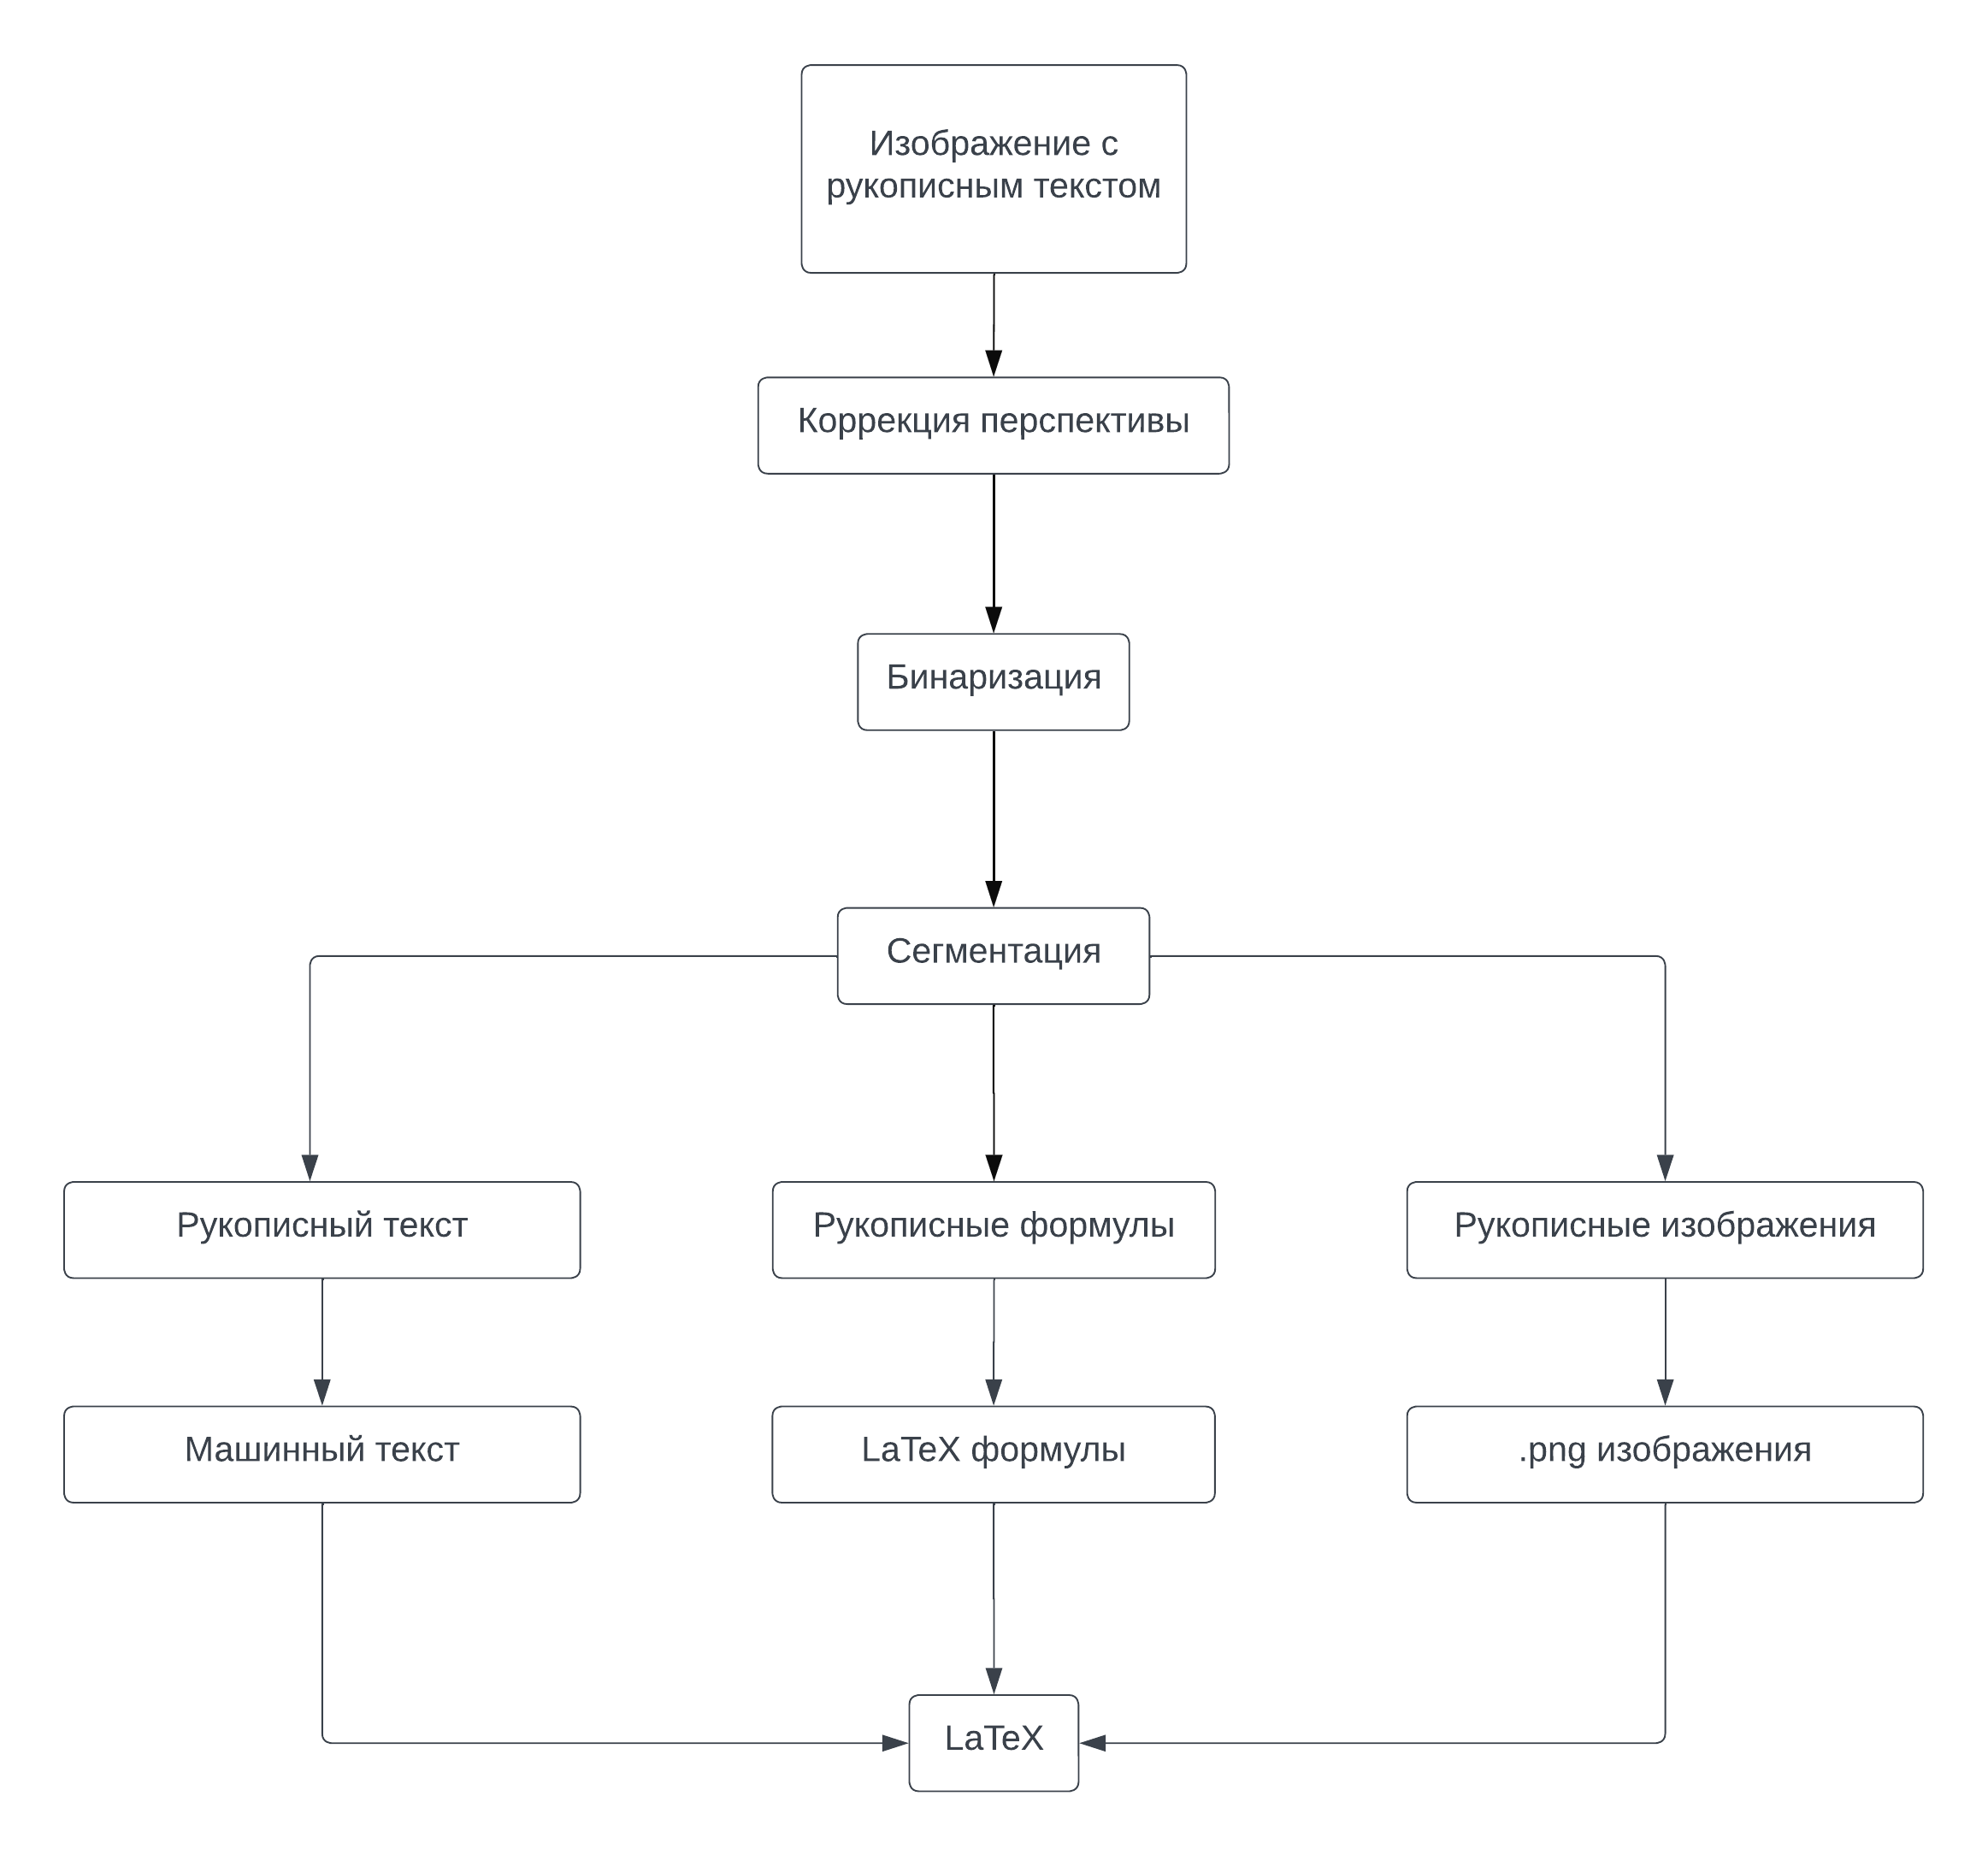
\includegraphics[scale=0.75]{img/Blank_diagram.png}
\caption{Общая архитектура модели}
\label{neuro_model}
\end{figure}

Подробнее разберем каждый этап данной схемы.
\subsection{Коррекция перспективы}

Коррекция перспективы необходима для устранения шума на изображении и получения лучшего результата. Она состоит из нескольких этапов, представленных на рисунке ~\ref{perspective_correction_algo}. 
Также на рисунке представлены результаты, получаемые на каждом из этапов обработки.

Стоит отметить, что коррекция перспективы осуществляется с использованием только алгоритмов обработки изображения без использования каких-либо нейросетей. 
Поэтому в целях экономии ресурсов сервера, а в следствии улучшения производительности было принято решение выполнять данный этап на машине клиента.
Схема данного алгоритма представлена на рисунке ~\ref{perspective_correction_algo}.
\begin{figure}
    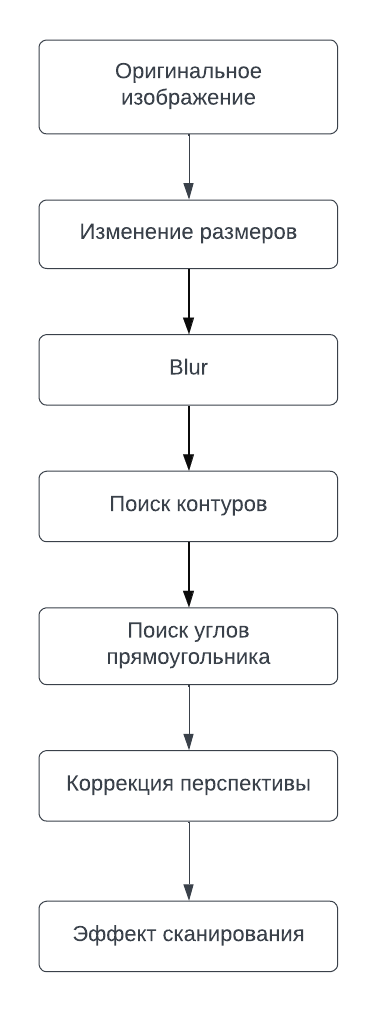
\includegraphics[scale=0.75]{img/perspective_correction}
    \caption{Этапы коррекции перспективы изображения}
    \label{perspective_correction_algo}
\end{figure}

На начальном этапе мы имеем изображение, показанное на рисунке ~\ref{input}

\begin{figure}
    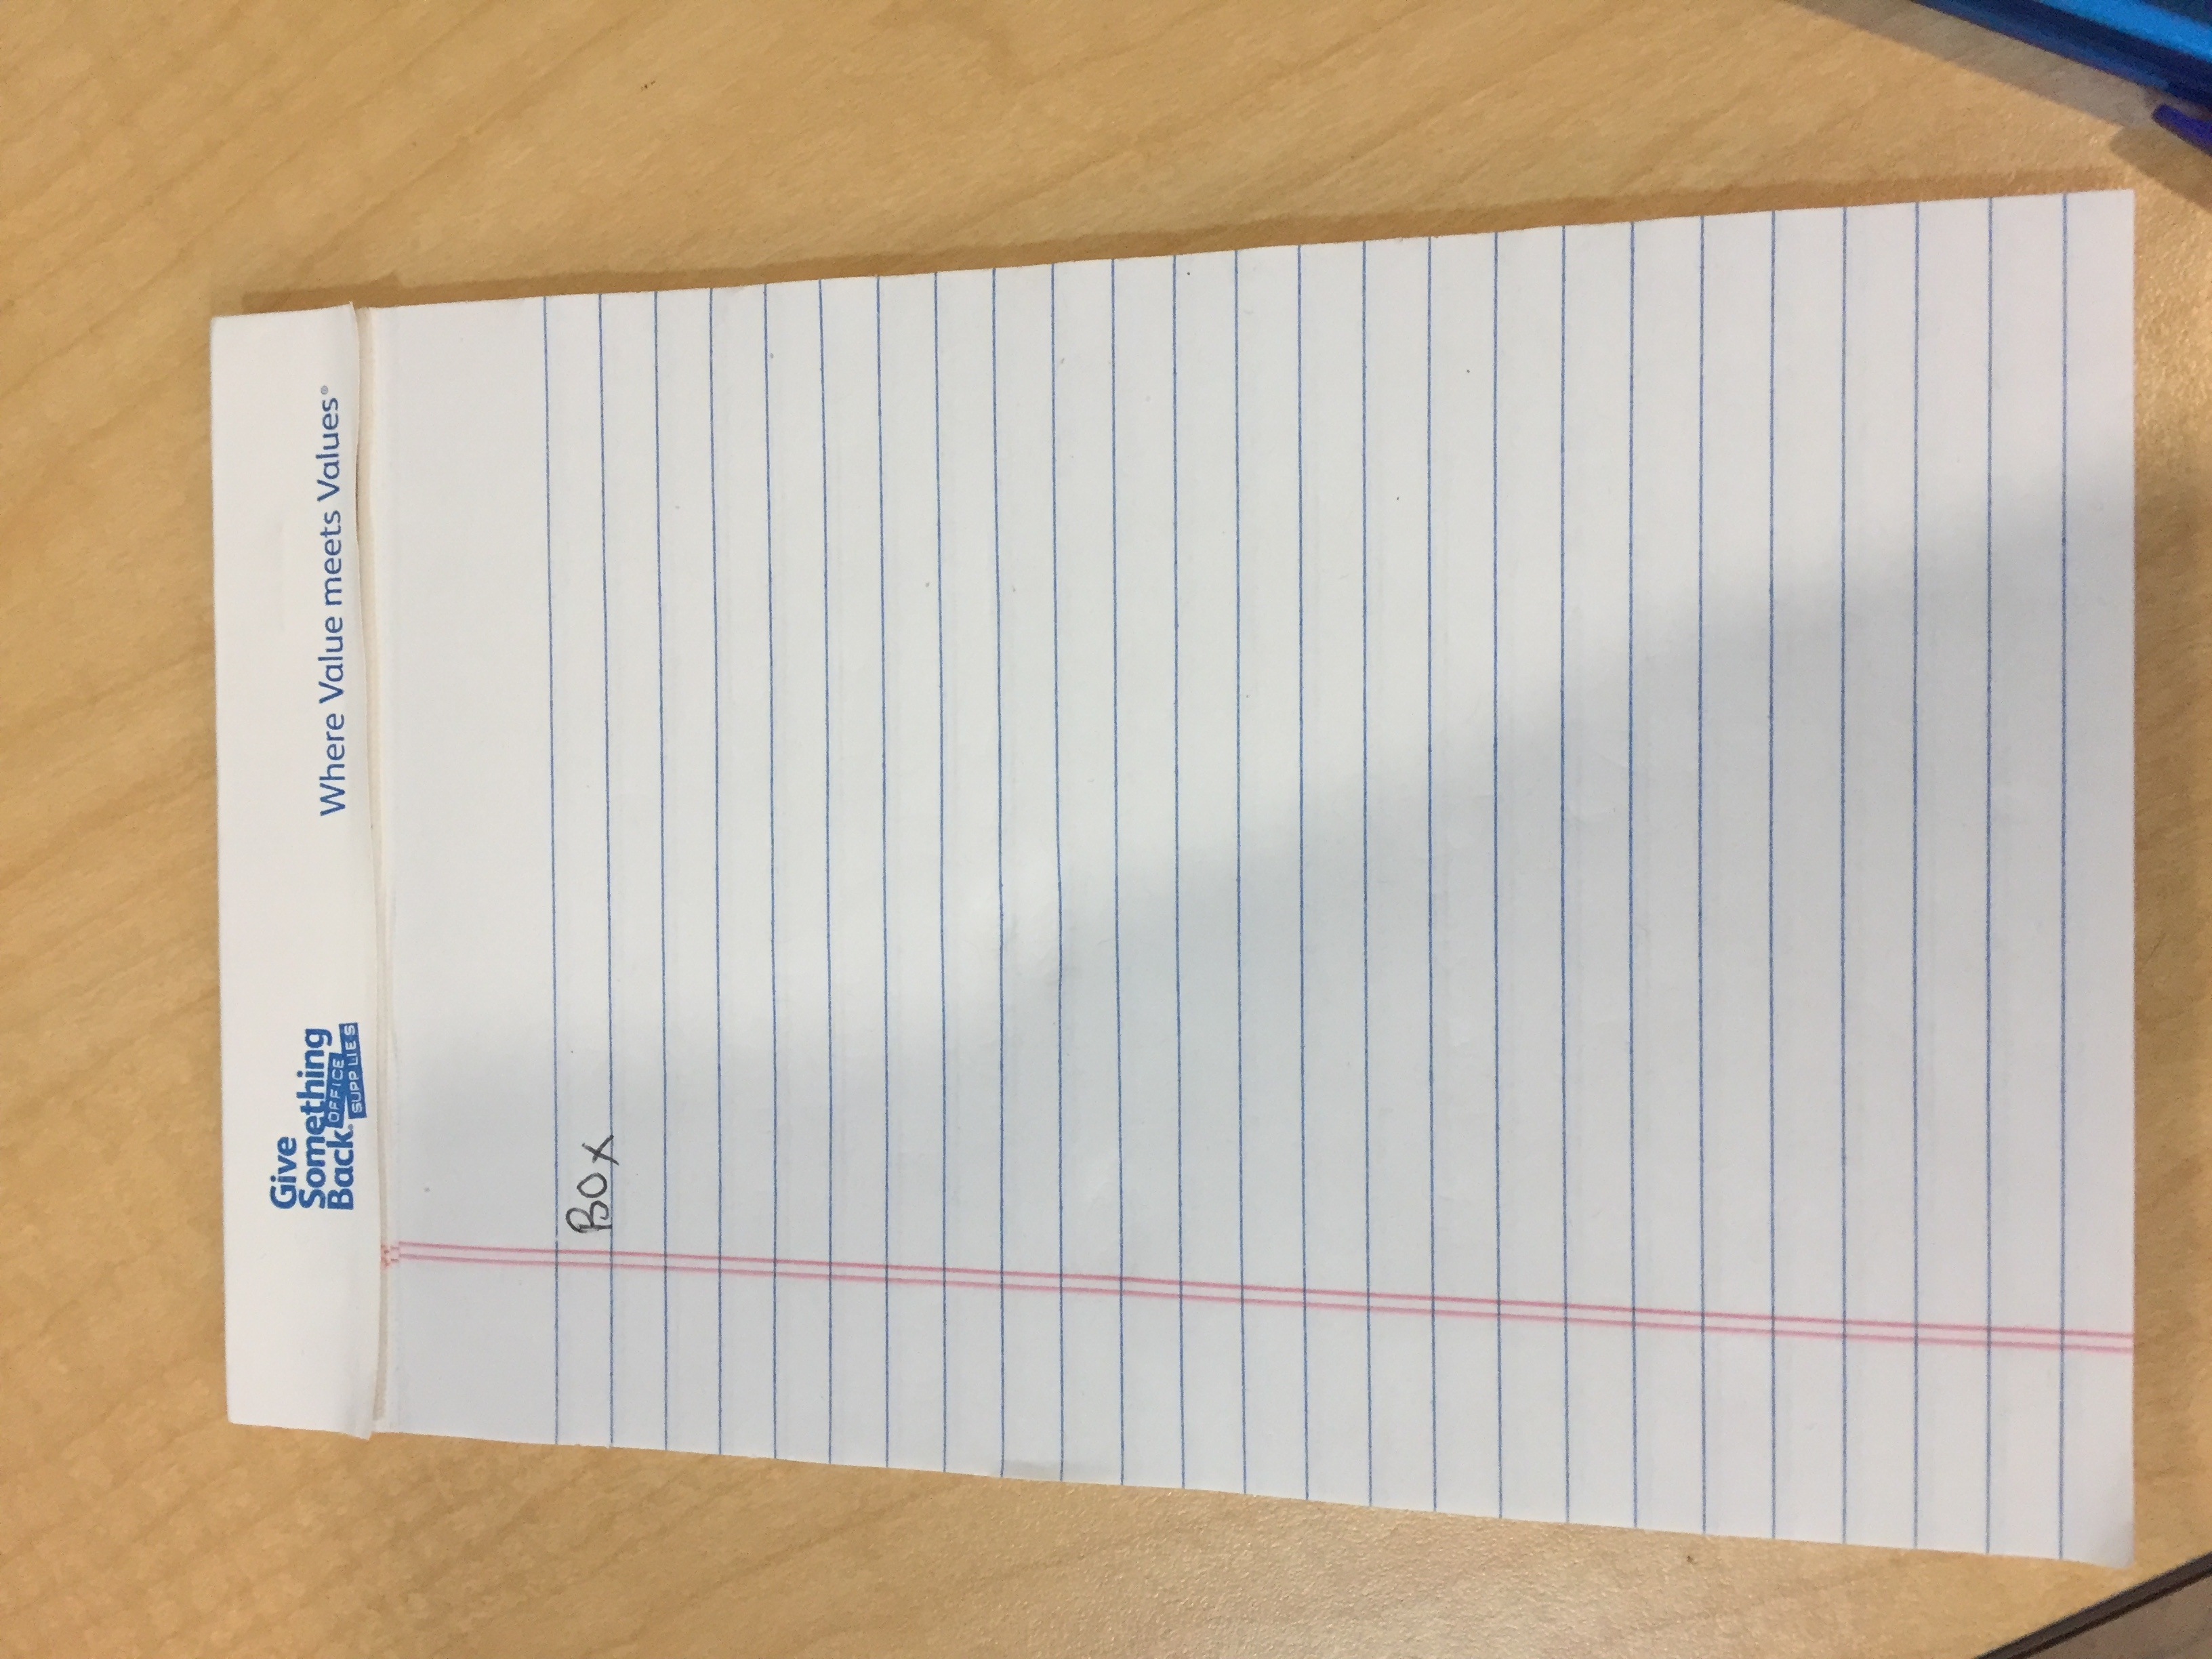
\includegraphics[scale=0.10]{img/perspective/input.JPG}
    \caption{Начальное изображение}
    \label{input}
\end{figure}

Для начала необходимо удалить текст с изображения. Для этого преобразуем изображение в серый цвет и применим к нему размытие Гаусса \cite{gauss_blur}. На выходе данного этапа имеем изображение, представленное на рисунке ~\ref{gauss_blur}

\begin{figure}
    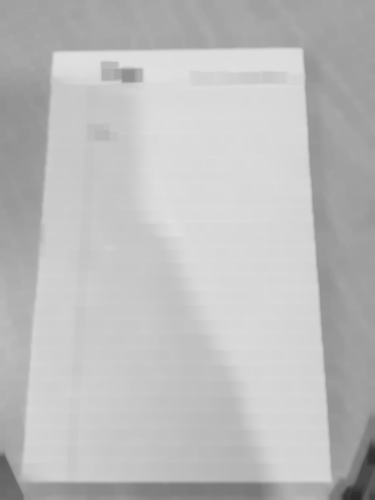
\includegraphics[scale=0.5]{img/perspective/blured.png}
    \caption{Изображение после размытия Гаусса}
    \label{gauss_blur}
\end{figure}

Для поиска контуров необходимо выделить ребра. Для этого используется алгоритм Канни \cite{canny}. На выходе имеем изображение, представленное на рисунке ~\ref{canny}
\begin{figure}
    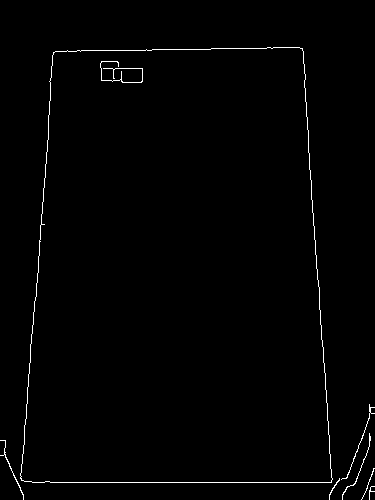
\includegraphics[scale=0.5]{img/perspective/canny.png}
    \caption{Ребра, найденные на изображении}
    \label{canny}
\end{figure}

После нахождения ребер поиск контуров осуществляется двумя способами:
\begin{enumerate}
    \item С помощью алгоритма $Line Segment Detector$ \cite{lsd}
    \item С помощью встроенного в $openCV$ алгоритма поиска контуров \cite{opencv_contours}
\end{enumerate}

Опишем подробнее поиск контуров на основе найденных линий: после прохода алгоритма имеем изображение, представленное на рисунке ~\ref{lsd_img}
\begin{figure}
    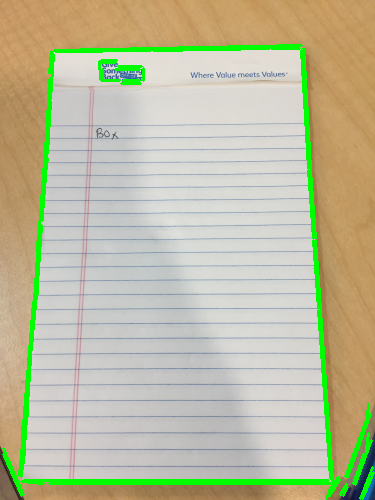
\includegraphics[scale=0.5]{img/perspective/lsd.png}
    \caption{Найденные на изображении линии с помощью алгоритма $LSD$}
    \label{lsd_img}
\end{figure}

Контур определяется как пересечение горизонтальных и вертикальных линий. На выходе имеем найденные углы контура, показанные на рисунке ~\ref{lsd_corners}
\begin{figure}
    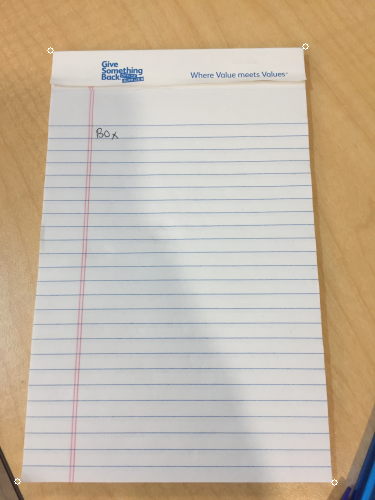
\includegraphics[scale=0.5]{img/perspective/corners.png}
    \caption{Найденные на изображении контуры на основе линий}
    \label{lsd_corners}
\end{figure}

С помощью библиотеки $openCV$ контуры находятся следующим образом:

\begin{enumerate}
    \item Находятся 5 наибольших по площади контуров
    \item Найденные контуры проверяются на количество углов, минимальную площадь контура
\end{enumerate}

Среди всех подходящих контуров выбирается наибольший по площади, как показано на рисунке ~\ref{contours}
\begin{figure}
    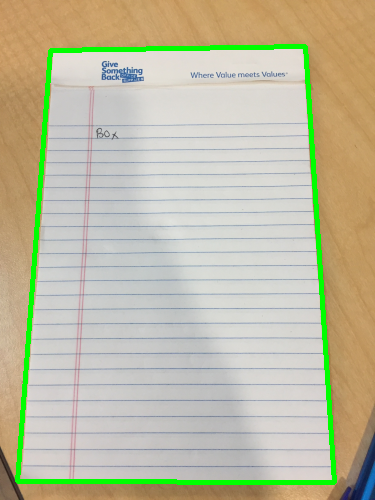
\includegraphics[scale=0.5]{img/perspective/contours.png}
    \caption{Найденные алгоритмом контуры}
    \label{contours}
\end{figure}


На основе найденного контура, представляющего лист бумаги, осуществляем коррекцию перспективы. Для этого находим матрицу коррекции \cite{opencv_perspective_transform} и примянем ее к изображению \cite{opencv_warp_perspective}.
Получаем результирующее изображение, показанное на рисунке ~\ref{perspective_correction}
\begin{figure}
    \includegraphics[scale=0.1]{img/perspective/perspective.png}
    \caption{Изображение с коррекцией перспективы}
    \label{perspective_correction}
\end{figure}

Далее необходимо добавить эффект сканирования. Эффект достигается путем применения к композиции небольшого размытия и серого изображения алгоритма сегментации $Adaptive Threshold$ \cite{opencv_threshold}. 
В конечном итоге имеем результирующее изображение показанное на рисунке ~\ref{preprocess_out}

\begin{figure}
    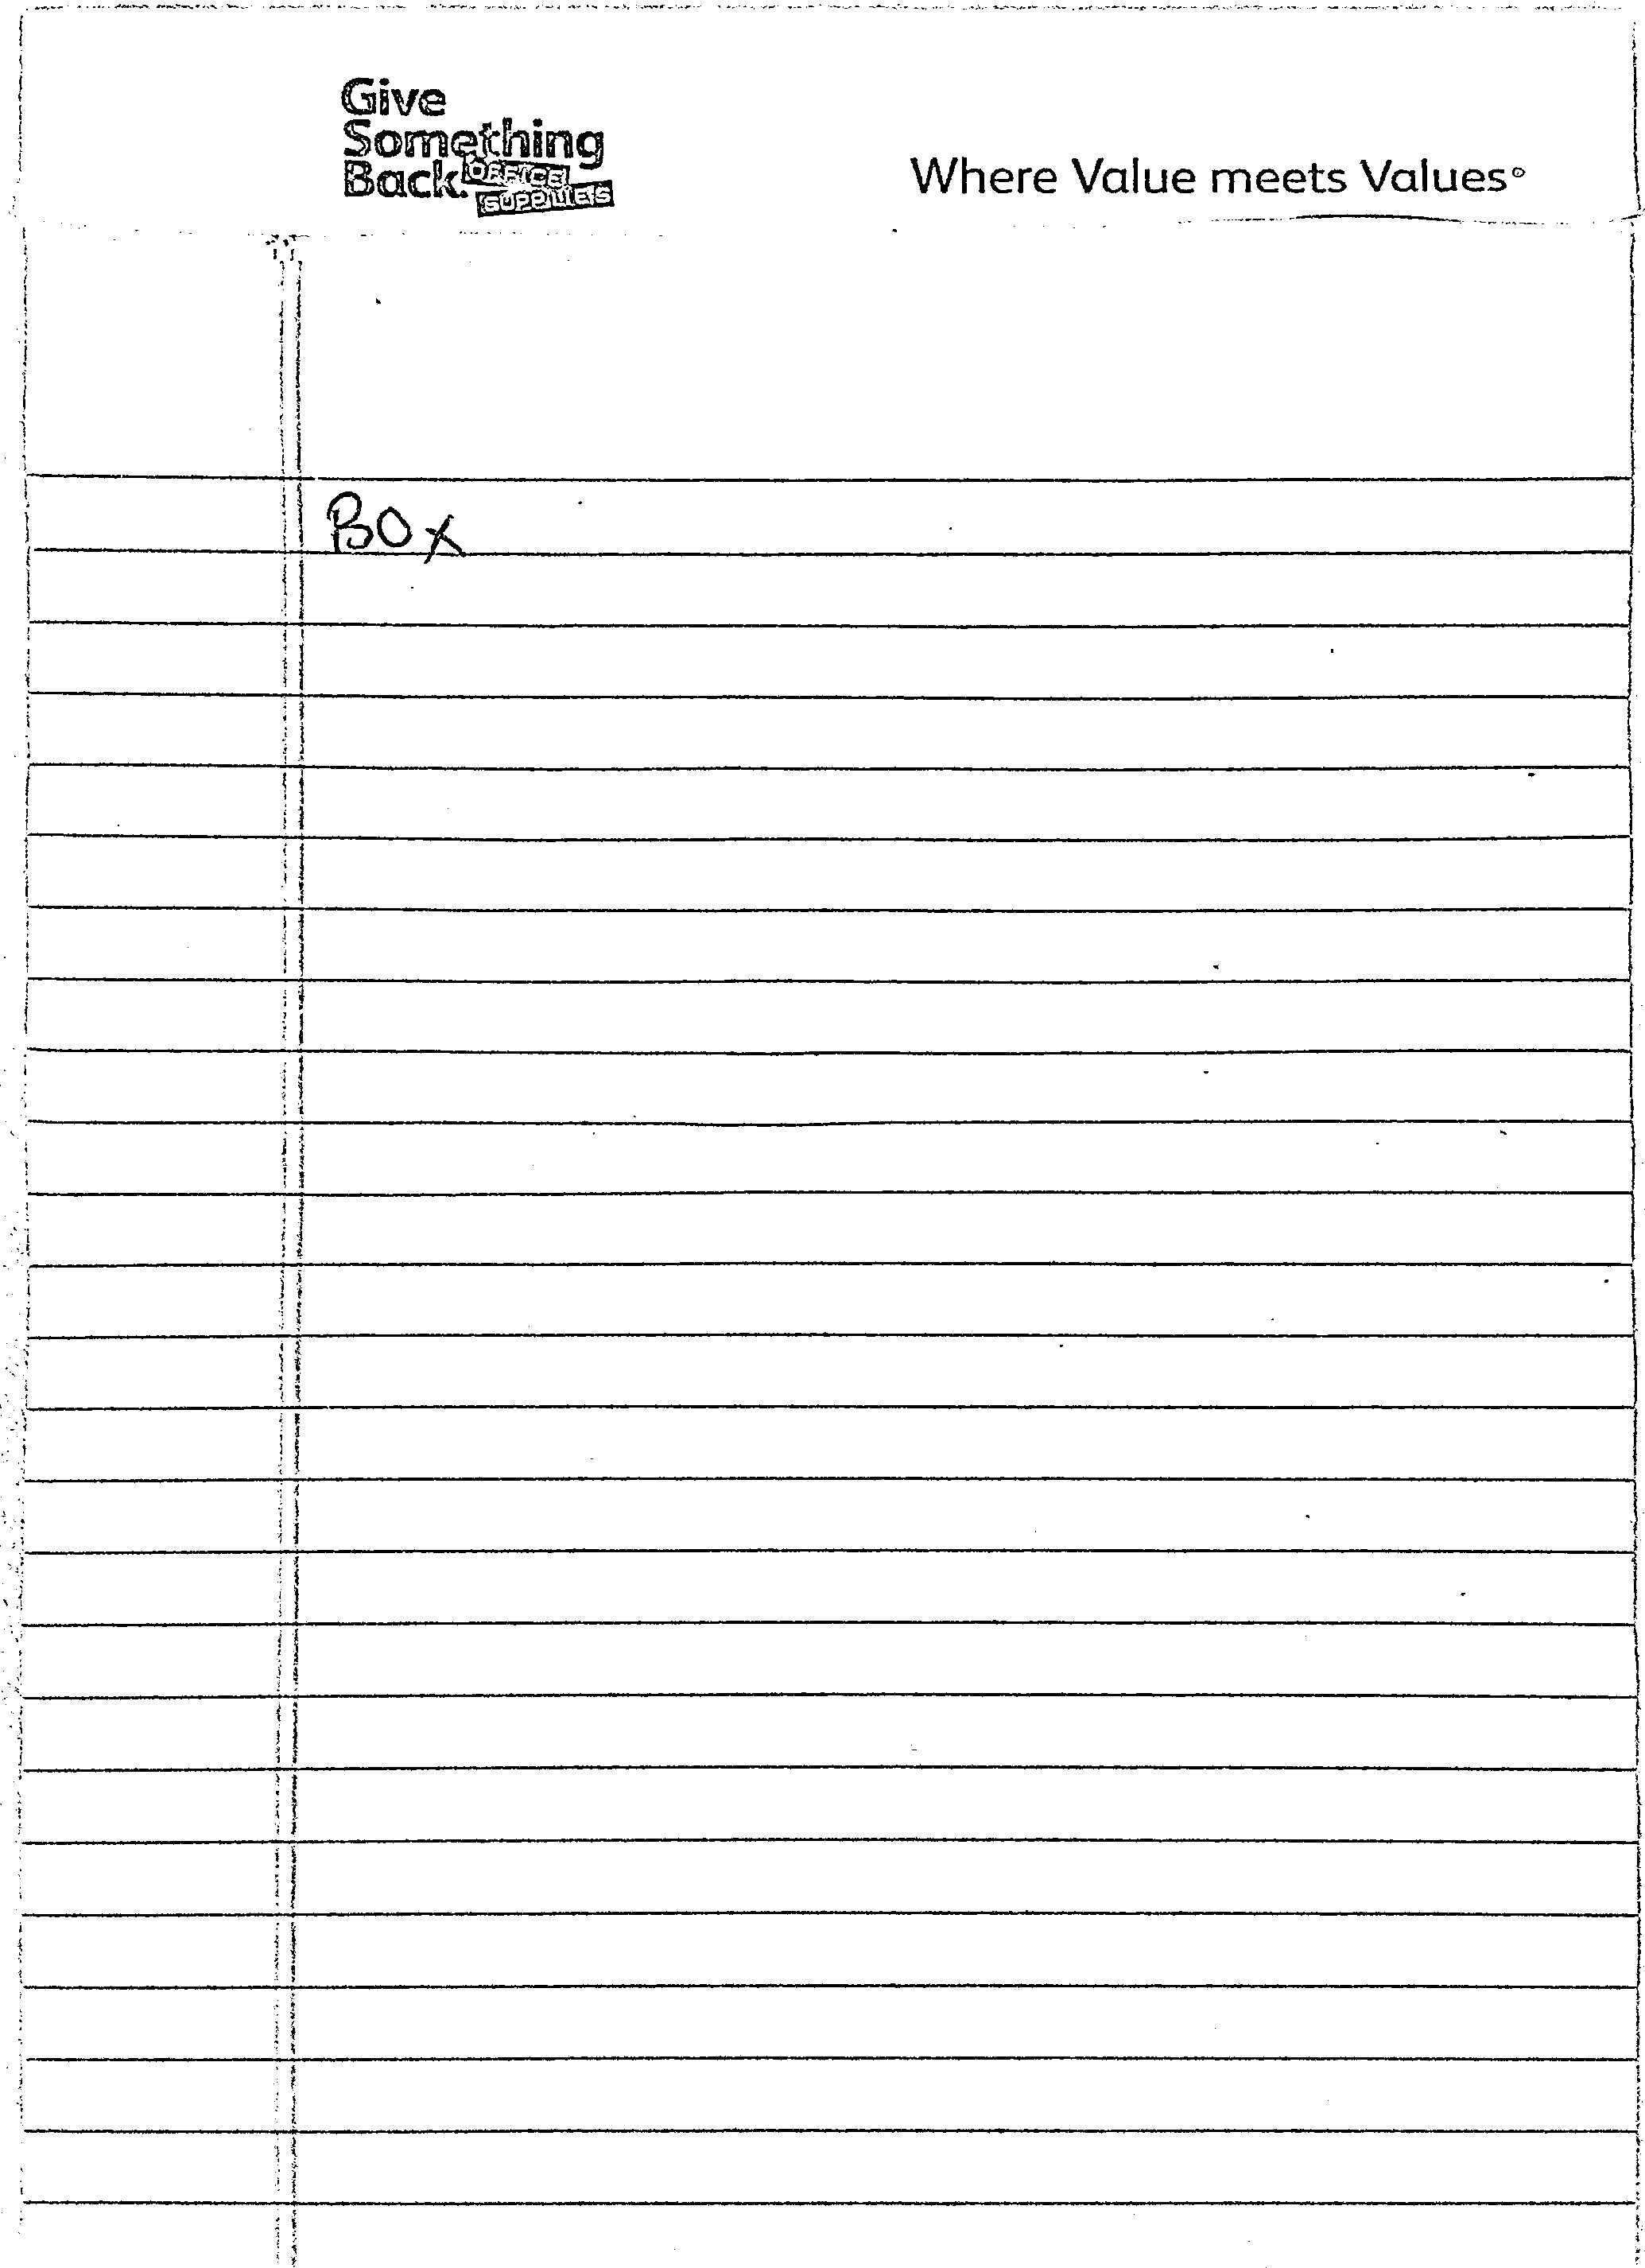
\includegraphics[scale=0.15]{img/perspective/output.JPG}
    \caption{Результирующее изображение}
    \label{preprocess_out}
\end{figure}

\subsubsection{Неправильное распознавание}
Стоит отметить, что данный алгоритм не является ультиимативным. Например, если на изображении находится посторонний шум (например, палец на бумаге, экран монитора, большое здание в виде прямоугольника), 
то алгоритм не сможет найти или найдет неверный контур. Именно с целью защиты от таких случаев в конечном продукте пользователь должен удостовериться в правильности найденного контура и отредактировать границы контура при необходимости.
Пример входного изображения, дающего неверный результат, и найденные на нем контуры приведены на рисунках ~\ref{perspective_wrong_input} и ~\ref{perspective_wrong_output} соответственно.

\begin{figure}
    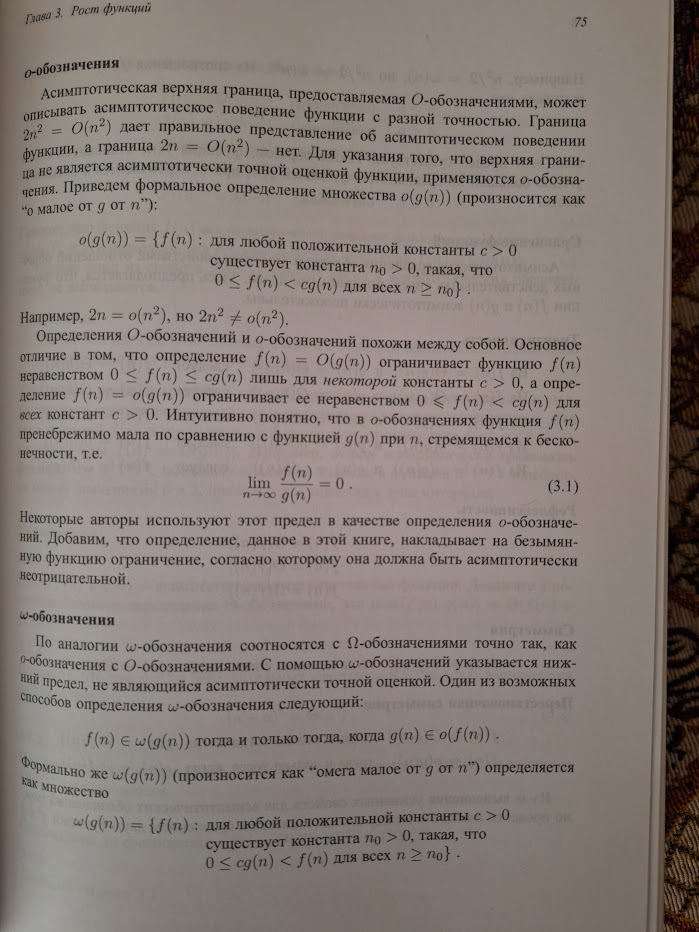
\includegraphics[scale=0.15]{img/perspective/wrong_input.JPG}
    \caption{Пример неправильно распозного изображения: входное изображение}
    \label{perspective_wrong_input}
\end{figure}

\begin{figure}
    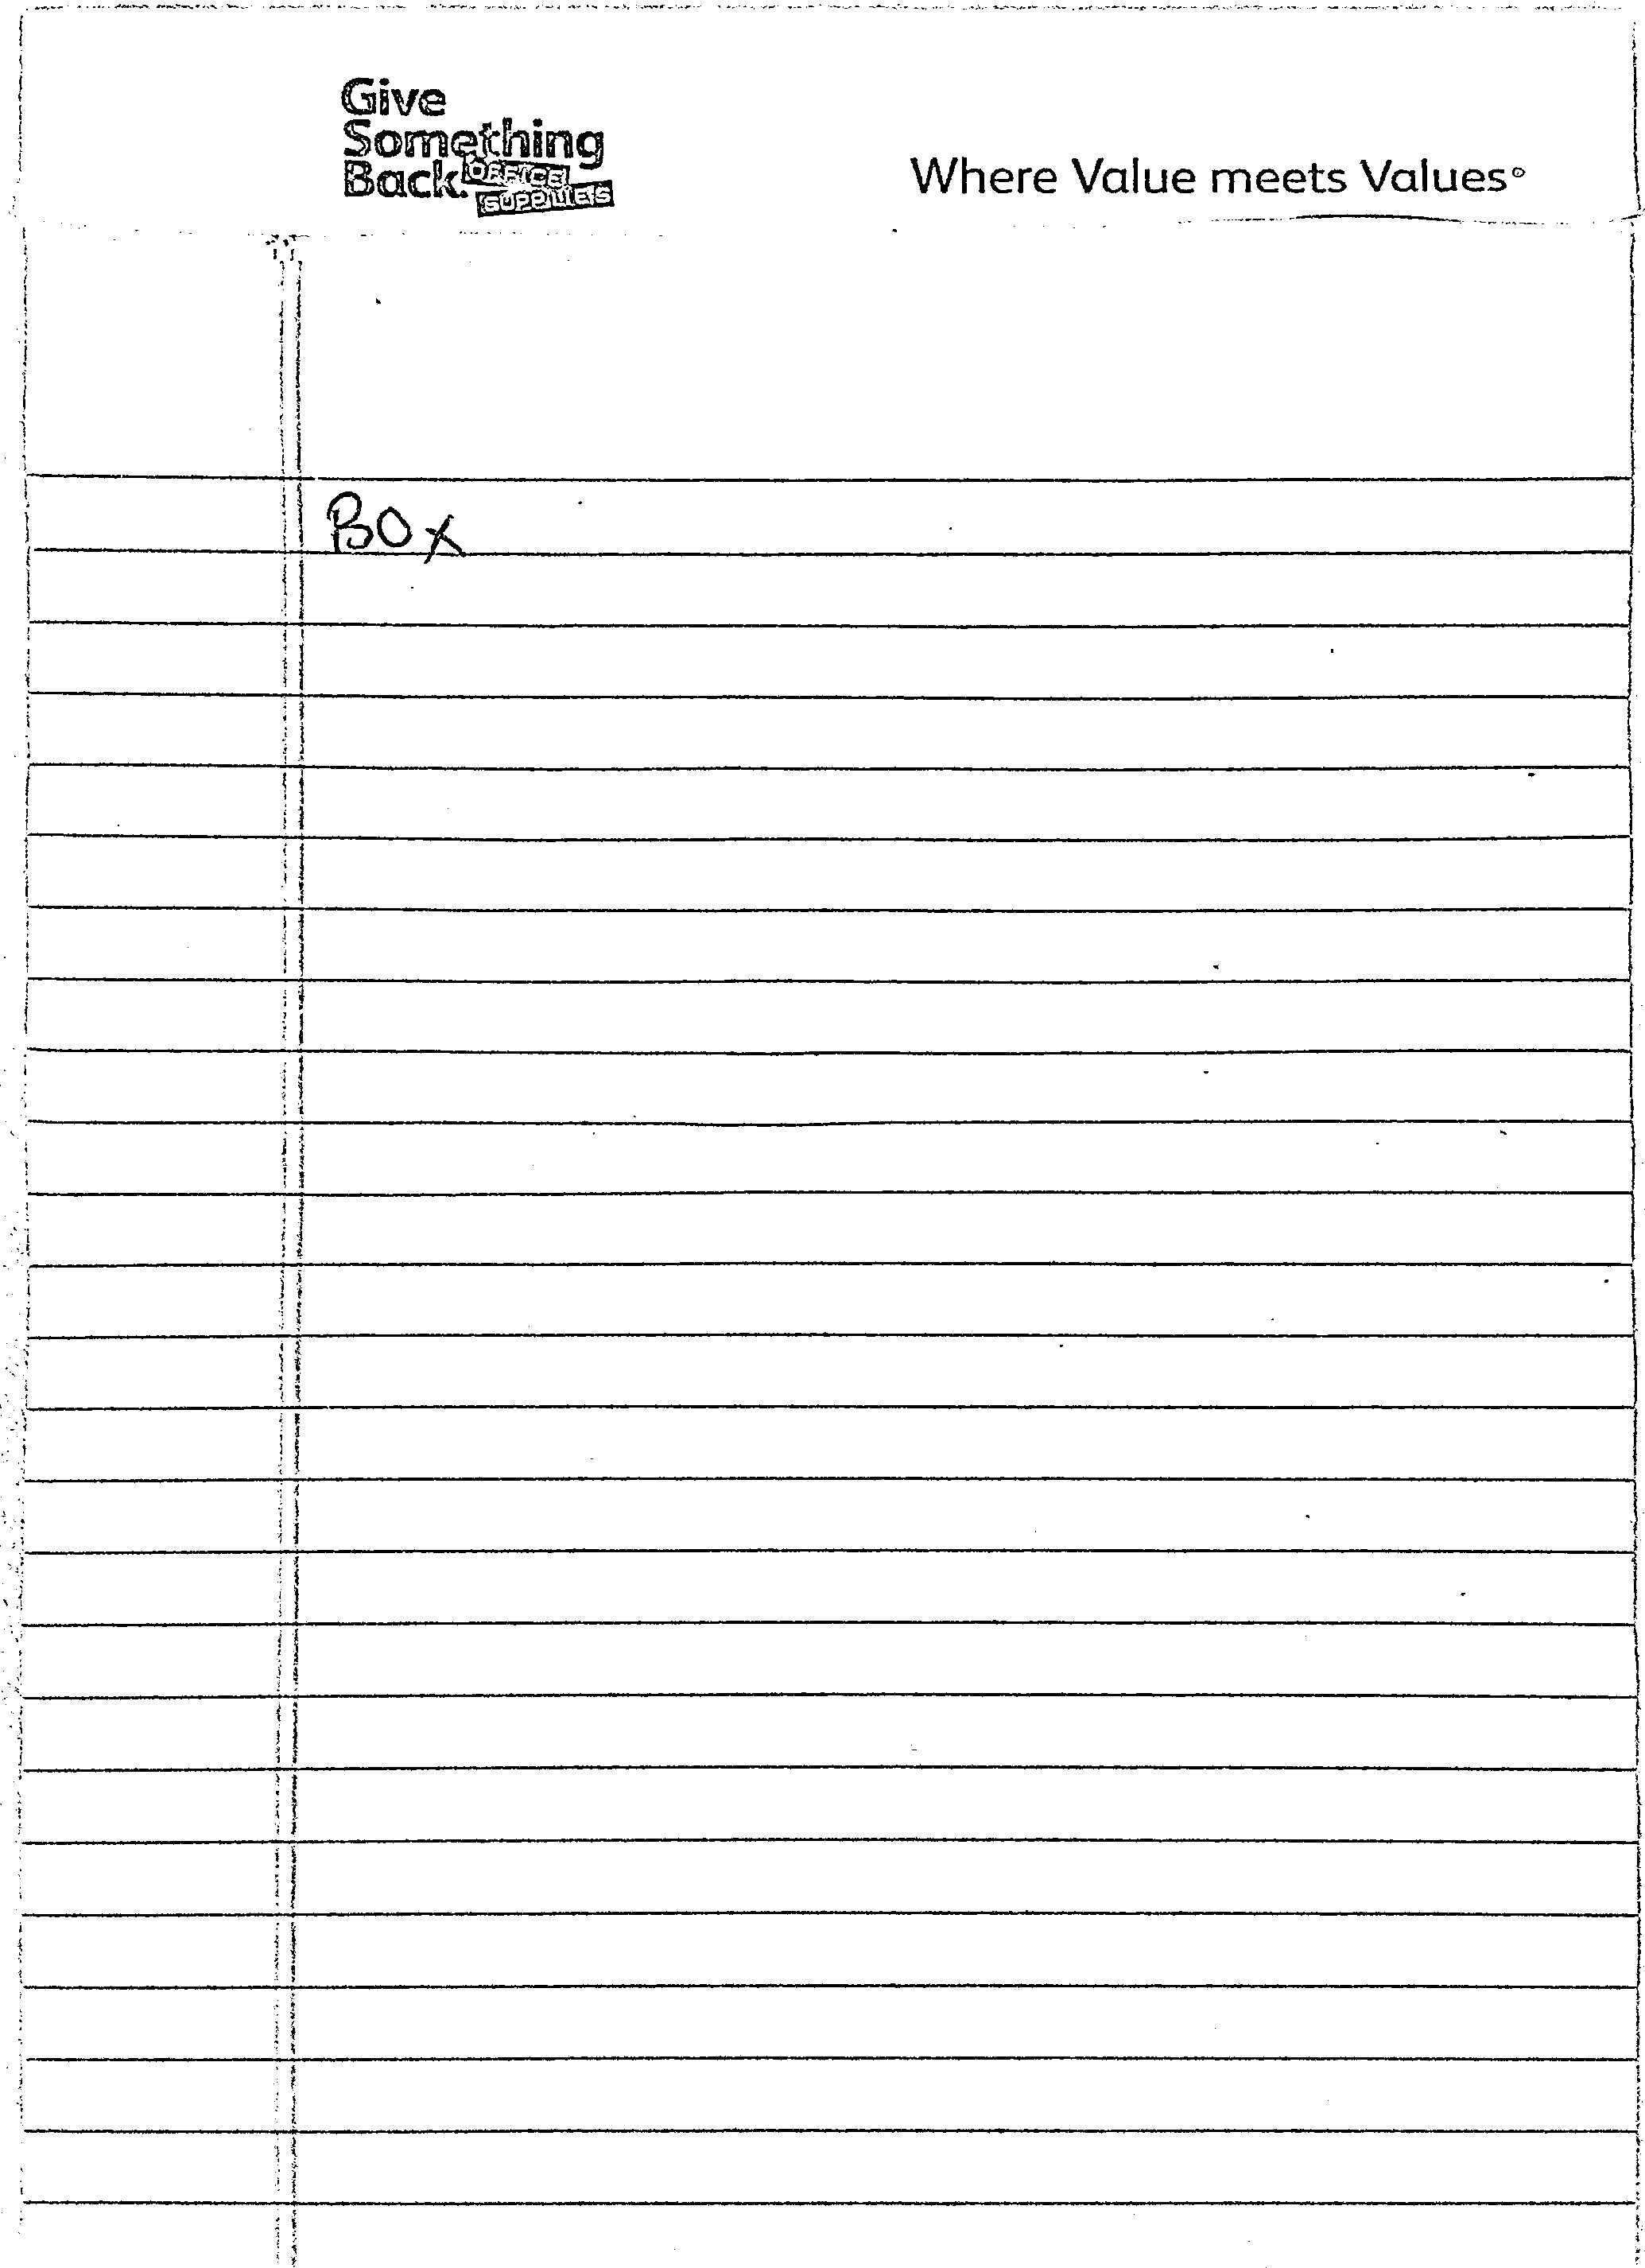
\includegraphics[scale=0.15]{img/perspective/wrong_output.JPG}
    \caption{Пример неправильно распозного изображения: найденные контуры}
    \label{perspective_wrong_output}
\end{figure}

\subsection{Сегментация}

Сегментация состоит из двух отдельных этапов:
\begin{itemize}
    \item Сегментация на абзацы
    \item Отделение текста от формул, рисунков и пр.
\end{itemize}

\subsubsection{Сегментация на абзацы}

Выделение абзацев требуется для их дальнейшего сохранения в \LaTeX\; коде. Данный вид сегментации, как и коррекция перспективы, осуществляется исключительно алгоритмически.
Поэтому данный этап можно также исполнять на машине пользователя.

%TODO: расписать сегментацию на абзацы
%TODO: Добавить пример неправильной сегментации

\subsubsection{Выделение формул}

Для выделения формул недостаточно одних алгоритмов обработки изображений. Существует множество моделей, выполняющих распознование объектов на изображении.
Одной из таких моделей является $YOLO$. Данная модель обладает следующими преимуществами:
\begin{itemize}
    \item Быстродействие. Нейросеть работает в реальном времени, поэтому её используют для распознавания объектов на фото и видео "здесь и сейчас".
    \item Точность. Нейросеть $YOLO$ умеет распознавать объекты разных размеров в пределах одного кадра.
    \item Универсальность. Нейросеть $YOLO$ способна определять как хорошо знакомые ей объекты, так и те, с которыми она ещё не сталкивалась.
    \item Простота. Модель $YOLO$ можно запросто запускать и дообучать с помощью $Tensorflow$.
\end{itemize}

Однако, данная модель не специализирована на какой-то одной задаче, поэтому будет проигрывать специализированным моделям.

На основании плюсов данной модели, а также на основании самой архитектуры системы, позволяющую при необходимости легко заменить выбранную модель на другую, было принято решение использовать для распознования формул модель $YOLO$ последней версии $v8$.

\subsubsection{Обучающие данные}
